\section{Identifying Subsystems}
As Capital Games exists as a website, a natural divison of subsystems arises: front end and back end. Front end essentially describes all the computations and objects that exist on the user's side of interaction with our application, and back end describes all the computations and objects that exist on the server's side. It is exceedingly simple to determine which parts of our system belong in the front end in the back end. We will also define another subsystem called "External" which will contain all the pieces necessary to our application but not technically a part of it. A high-level view of our system in the form of ``packages'' or subsystems follows on one of the next few pages. \\

As it turns out, we can go deeper into our system to define subsystems within the back end. Though the front end is relatively simple, the back end of our system is where most of the computation and interesting events occur. There are two major subsystems as have been described in previous sections of this report: financial data retrieval and the queueing subsystems. In addition to these two subsystems, the database and the controller exist within the back end, but it does not seem appropriate to further include them in another subsystem, as they are essentially separate, stand-alone packages that interact with or call upon the other packages within the system. \\

The financial data retrievial subsystem is the simpler of our two subsystems. It only requires the ability to handle requests given to it by the controller (requests ultimately generated by a user) and the ability to fetch data from Yahoo! Finance in response to a valid request. The queuing system is only somewhat more complicated, needing background processes to monitor outstanding tasks, an Action Mailer object to handle sending e-mails to users, and an order handler that can understand and process orders. Though the controller facilitates all their interactions with the rest of the system, these two packages dominate most of our application design and are the backbone of its functionality. \\ \\ \\ \\ \\ \\ \\ \\

\begin{figure}[H]
\centering
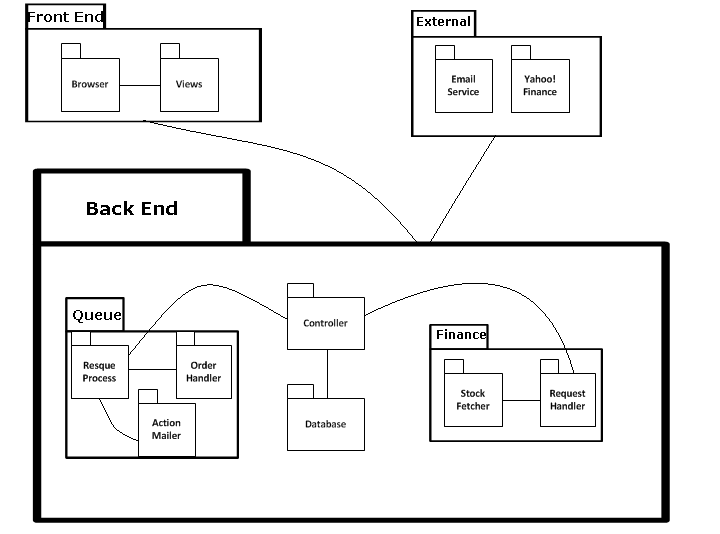
\includegraphics[width=7in]{./img/package.png}
\caption{The UML package diagram for our system.}
\end{figure}
